% Shared standalone design for the editable figure reconstructions.
\documentclass[tikz,border=5pt,10pt]{standalone}
\usepackage[T1]{fontenc}
\usepackage[utf8]{inputenc}
\usepackage{newpxtext,newpxmath}
\usepackage[scaled=.94]{sourcesanspro}
\usepackage{pgfplots}
\pgfplotsset{compat=1.18}
\usetikzlibrary{arrows.meta,calc,positioning,decorations.pathreplacing,
  decorations.markings,patterns,matrix,shapes.geometric,fit,backgrounds,
  intersections,angles,quotes}
\definecolor{ink}{HTML}{203746}
\definecolor{accent}{HTML}{146C78}
\definecolor{muted}{HTML}{667780}
\definecolor{signalred}{HTML}{B94B44}
\color{ink}
\tikzset{>=Latex,line width=.8pt,
  every node/.style={font=\small},
  axis/.style={->,draw=muted,line width=.5pt},
  guide/.style={draw=muted,dashed,line width=.45pt},
  curve/.style={draw=accent,line width=1pt},
  marker/.style={circle,fill=accent,inner sep=1.5pt},
  labelbox/.style={fill=white,inner sep=2pt}}

\begin{document}
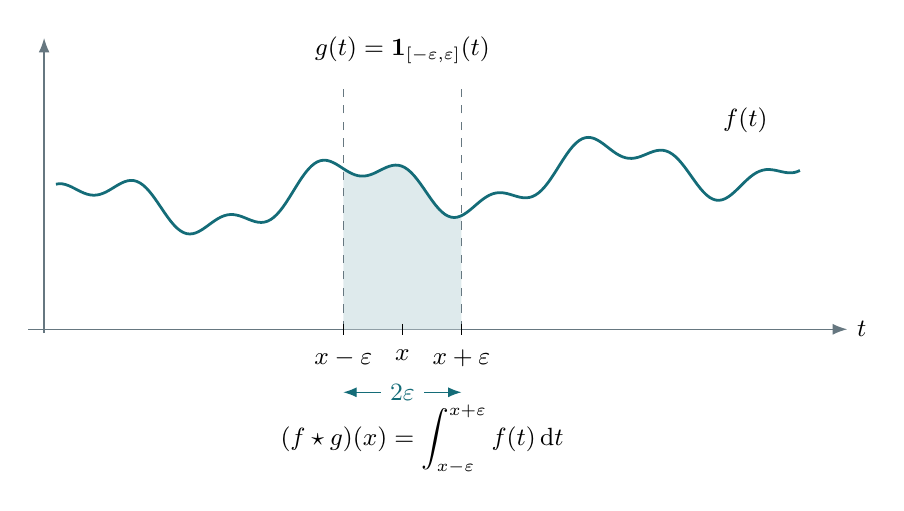
\begin{tikzpicture}[x=1cm,y=1cm]
\draw[axis] (0,0)--(10.4,0) node[right] {$t$};
\draw[axis] (.2,-.05)--(.2,3.7);
\fill[accent!14] plot[domain=4.0:5.5,samples=70] (\x,{1.45+.075*\x+.35*sin(110*\x)+.16*sin(320*\x)}) -- (5.5,0)--(4,0)--cycle;
\draw[curve,domain=.35:9.8,samples=240] plot (\x,{1.45+.075*\x+.35*sin(110*\x)+.16*sin(320*\x)});
\draw[guide] (4,0)--(4,3.15) (5.5,0)--(5.5,3.15);
\node[anchor=south] at (4.75,3.25) {$g(t)=\mathbf{1}_{[-\varepsilon,\varepsilon]}(t)$};
\node[anchor=west] at (8.7,2.65) {$f(t)$};
\foreach \x/\lab in {4/{x-\varepsilon},4.75/{x},5.5/{x+\varepsilon}} {
 \draw (\x,.07)--(\x,-.07); \node[below] at (\x,-.13) {$\lab$};}
\draw[<->,accent] (4,-.8)--node[fill=white] {$2\varepsilon$}(5.5,-.8);
\node at (5,-1.4) {$(f\star g)(x)=\displaystyle\int_{x-\varepsilon}^{x+\varepsilon}f(t)\,\mathrm{d}t$};
\end{tikzpicture}
\end{document}
